\subsection{Qt's object model}

\begin{frame}
  \frametitle{Qt's object model -- \texttt{QObject}\footnote
    {http://doc.qt.io/qt-5.6/qobject.html}}
  \begin{itemize}
    \item Common base class for many classes in Qt.
    \item \texttt{QObject} adds several fundamental features used throughout
      the rest of Qt:
    \begin{itemize}
      \item dynamic properties,
      \item the signals and slots mechanism,
      \item event handling,
      \item the memory management model,
      \item basic run-time reflection -- metaobject system.
    \end{itemize}
    \item Some of the features are implemented by employing an external
      code-generator the metaobject compiler -- \texttt{moc}.
    \item \texttt{QObject} is {\em not} responsible for the visual representation.
    \begin{itemize}
      \item This is the responsibility of \texttt{QWidget}\footnote{More on that
      later} and its descendants.
    \end{itemize}
  \end{itemize}
\end{frame}

\begin{frame}
  \frametitle{\texttt{QObject} tree}
  \begin{itemize}
    \item \texttt{QObject}s are usually organized in a N-way tree hierarchy.
    \begin{itemize}
      \item Each instance of \texttt{QObject} has either zero\footnote{the tree root}
      or one\footnote{the inner nodes or leaves} {\em parent} \texttt{QObject}.
      \item Each \texttt{QObject} has zero or N {\em child} \texttt{QObject}s.
      \item {\em Not to be confused with class inheritance hierarchy!}
    \end{itemize}
    \item The \texttt{QObject}s implements {\em memory management}:
    \begin{itemize}
      \item Each parent is responsible for the lifetime management of its
      child nodes.
    \end{itemize}
    \item The children of a \texttt{QObject} can be iterated -- the whole tree
      can be traversed.
  \end{itemize}
\end{frame}

\begin{frame}
  \frametitle{Class inheritance vs. \texttt{QObject} ownership}
  \begin{columns}
    \begin{column}{0.47\textwidth}
    \begin{figure}[!t]
    \centering
    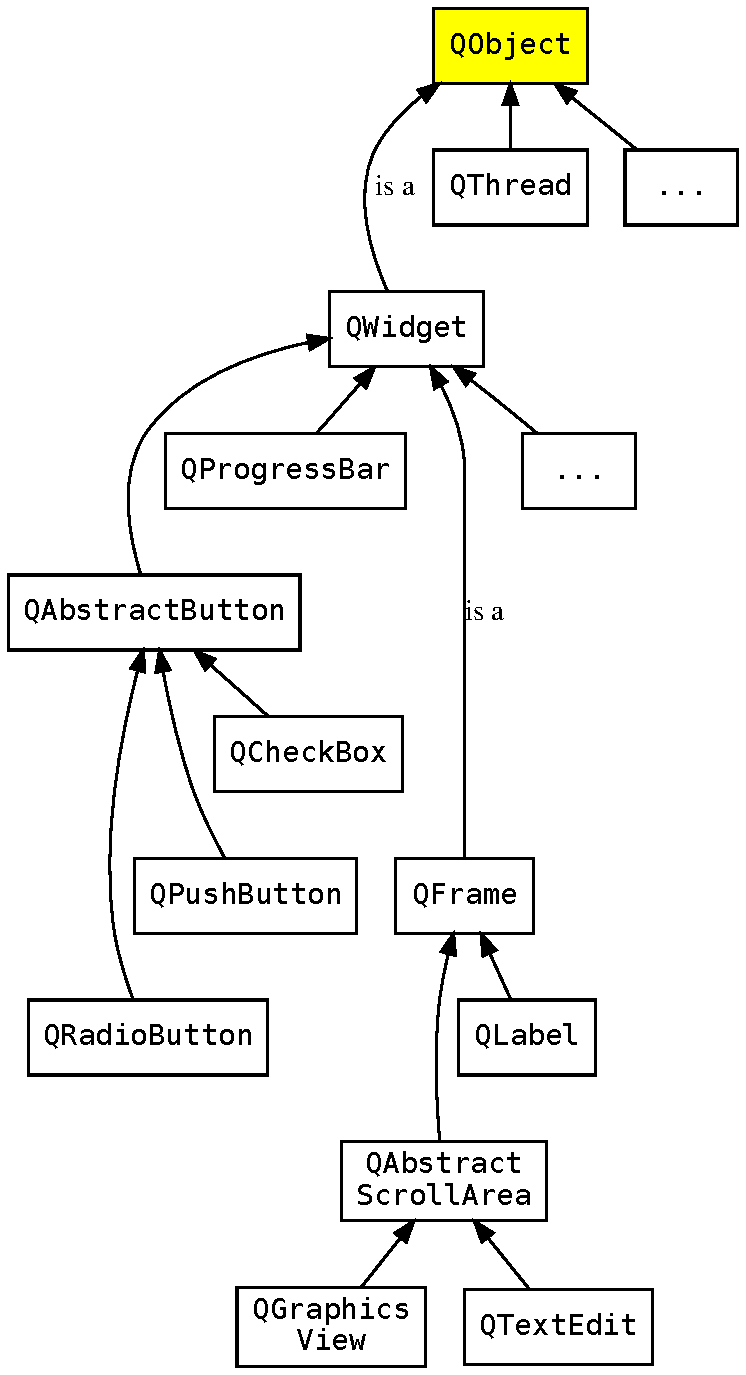
\includegraphics[height=0.72\textheight]{images/class_tree.pdf}
    \caption{\footnotesize Class inheritance hierarchy}
    \end{figure}
    \end{column}
    \begin{column}{0.52\textwidth}
    \begin{figure}[!t]
    \centering
    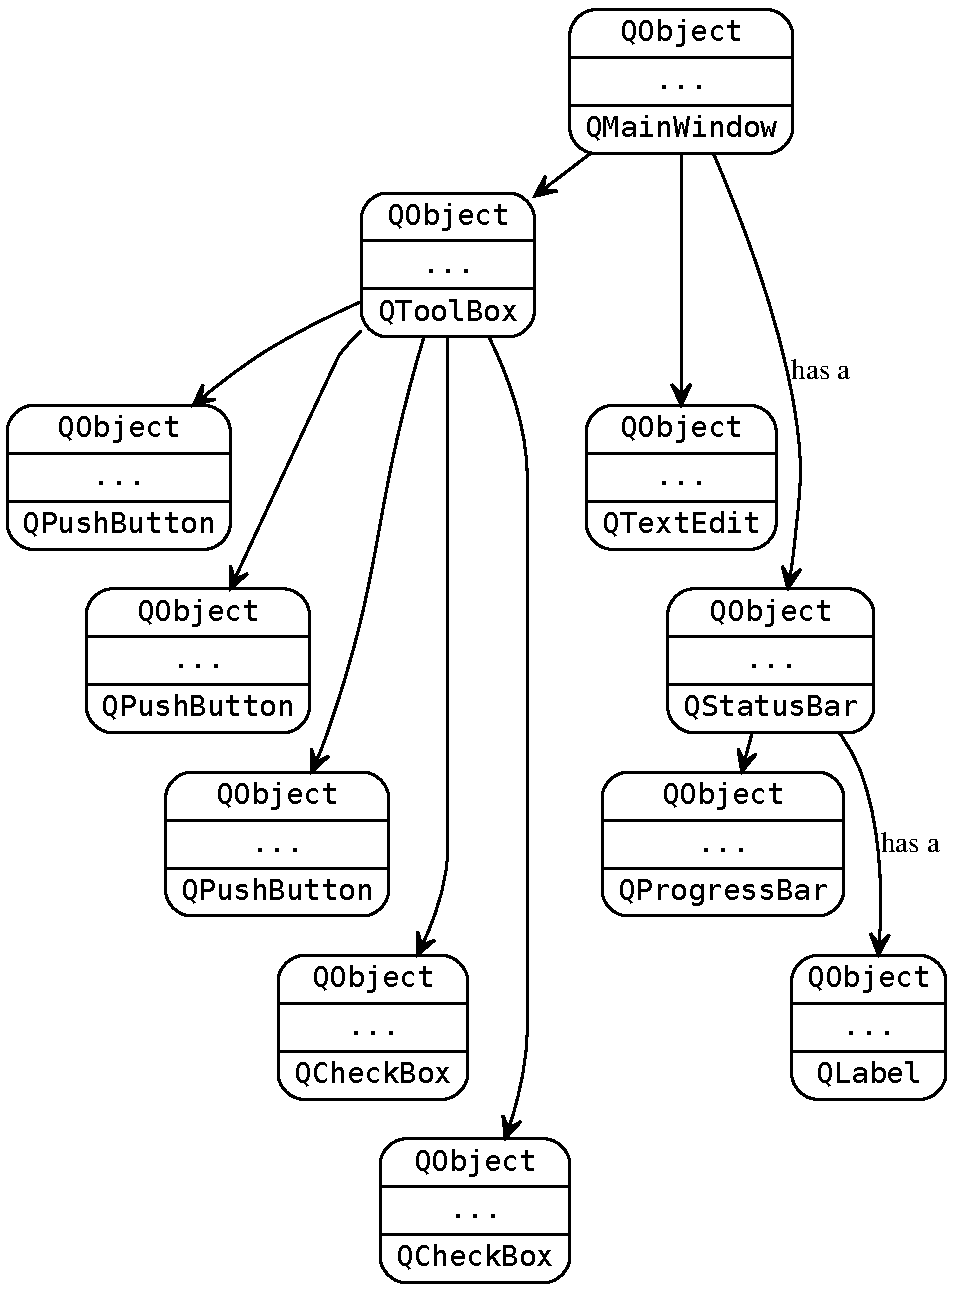
\includegraphics[height=0.72\textheight]{images/qobject_tree.pdf}
    \caption{\footnotesize \texttt{QObject} ownership hierarchy}
    \end{figure}
    \end{column}
  \end{columns}
\end{frame}

\begin{frame}
  \frametitle{\texttt{QObject} -- memory management}
  \begin{itemize}
    \item Instances of \texttt{QObject} are for the most part\footnote{except
      for the roots} dynamically allocated.
    \item The parent -- child relationship is usually created when the child
    node instance is constructed:
    \begin{itemize}
      \item The parent node is assigned to the child \texttt{QObject},
        in the child's constructor -- as one of its parameters.
      \item The child node is also added to the list of children of the parent
        \texttt{QObject} during its construction.
    \end{itemize}
    \item Each parent {\em owns} its child \texttt{QObject} instances.
    \item \texttt{QObject} disables copy-construction.
  \end{itemize}
\end{frame}

\begin{frame}
  \frametitle{\texttt{QObject} -- memory management}
  \begin{itemize}
    \item When the parent instance of \texttt{QObject} is destroyed, it also
      deletes all of its children.
    \begin{itemize}
      \item The memory allocation \footnote{calling \texttt{new}} is
        usually done manually.
      \item The deallocation\footnote{calling \texttt{delete}} is mostly automated.
    \end{itemize}
    \item If used properly and consistently then;
    \begin{itemize}
      \item each object is deleted -- no memory leaks,
      \item object is deleted exactly {\em once} -- no memory access violations.
    \end{itemize}
  \end{itemize}
\end{frame}

\begin{frame}[fragile]
  \frametitle{Allocating memory for instances of various types}
  \small
  \begin{itemize}
    \item Specializations of \texttt{QObject}
    \begin{itemize}
      \item Usually allocated on the heap:
      \begin{verbatim}
	QPushButton* btn = new QPushButton("OK", parent);
      \end{verbatim}
      \item Except:
      \begin{itemize}
        \item classes with lifetimes spanning the whole run-time of the
        application 
        \begin{verbatim}
	QApplication(argc, argv);
	QMainWindow mainWin(...);
        \end{verbatim}
        \item or used as temporary variables in functions:
        \begin{verbatim}
	QFileDialog fileDlg(...);
	QFile file(...);
        \end{verbatim}
      \end{itemize}
    \end{itemize}
  \end{itemize}
\end{frame}

\begin{frame}[fragile]
  \frametitle{Allocating memory for instances of various types}
  \begin{itemize}
    \item All other classes
    \begin{itemize}
      \item Usually allocated on the stack:
      \begin{verbatim}
	QString str;
	QByteArray ba = str.toUtf8();
	QStringList strlist;
	QSet<QString> set;
	QMap<int, QString> map;
	QHash<int, QString> hmap;
	QColor color;
	QDir dir;
	// etc.
      \end{verbatim}
      \item Optimized for cheap copying.
    \end{itemize}
  \end{itemize}
\end{frame}

